\cotefile{15}
\scanpage{59}
Catégories de Deuring.

1. Catégories $A$-linéaires et $\otimes$-enveloppes.

$A$ est un annea\unsure{\deleted{t}u|\deleted{u}t|b} commutatif. Soit $C$ une catégorie $A$-linéaire (i.e. les $\operatorname{Hom}$ dans $A$ sont des $A$-modules, l'accouplement des $\operatorname{Hom}$ étant bilinéaire). Un \unsure{\deleted{h}f|\deleted{f}h}oncteur $A$-linéaire
\[
F:\ C\handwritten{\longrightarrow}C'
\]
de $C$ dans une autre catégorie $A$-linéaire $C'$ est dit \inserted{``admissible'' ou} ``compatible au produit tensoriel externe'' si pour tout objet $X$ de $C$ sur lequel opère ($A$-linéairement) une $A$-algèbre $o$, et tout $o$-module à droite $P$ tel que $P\otimes_o X$ existe dans $C$, $\deleted{\unsure{F(}}P\deleted{)}\otimes_o F(X)$ existe dans $C'$ et l'homomorphisme naturel
\margin{\figure{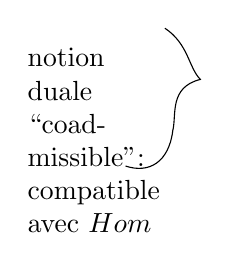
\begin{tikzpicture}[x=1cm,y=1cm]
\node[anchor=north west,text width=1.7cm,inner sep=0pt] at (0,0) {notion duale ``coadmissible'': compatible avec $\operatorname{Hom}$};
\handwritten{\draw (1.75,.25) .. controls (2.05,.05) and (2.05,-.25) .. (2.2,-.4) .. controls (1.8,-.5) and (1.9,-.85) .. (1.85,-1.05) .. controls (1.8,-1.45) and (1.55,-1.6) .. (1.25,-1.5);}
\end{tikzpicture}}}
\[
P\otimes_o F(X)\handwritten{\unsure{\text{---}|\longrightarrow}}F(P\otimes_o X)
\]
est un isomorphisme. Si $C$ est une catégorie de Deuring, alors il suffit de poser cette condition pour un objet fixé $X$ de $C$, et pour $o=\operatorname{End}_C(X)$, $P$ un module $\handwritten{\in}\uline{P}(\unsure{o/A})=$ catégorie des $o$-modules à droite qui sont localement sur $S=\operatorname{Spec}(A)$ libres de rang $1$. Dans ce cas, la catégorie des foncteurs $F$ en question est équivalente, par
\margin{\handwritten{il suffit que $C$ \unsure{admette} $X$ \deleted{\unsure{comme|un}} ``générateur strict'': \unsure{tt} objet de $C$ de la forme $P\otimes_o X$, et que \unsure{avec} $P$ projectif de type fini, alors équiv. $\uline{P}\longmapsto P\otimes_o X$ (\unsure{sur ss-cat} $\unsure{\mathbb{P}(o)X|P(o)X}$) (pour $P\otimes_o X$ \unsure{existe})}}
\margin{\handwritten{$P\otimes_o X\overset{\sim}{\longrightarrow}\operatorname{Hom}_o(\check P,X)$}}
\[
F\handwritten{\longmapsto}F(X)\ :\ \uline{\operatorname{Hom}}_{A\text{-}\mathrm{adm}}(C,C')\handwritten{\hookrightarrow}\operatorname{Mod}(o,C'),
\]
à la catégorie des objets \inserted{$X'$} de $C'$ avec opération \inserted{$A$-linéaire de} de $o$, tels que $P\otimes_o X'$ exist dans $C'$ pour tout $P\handwritten{\in}\operatorname{ob}\uline{P}(o/A)$. En tous cas, la catégorie des foncteurs admissibles de $C$ dans $C'$ est $A$-linéaire.

\inserted{Soit}
\[
\deleted{\text{Soit}}\quad C(1)=\uline{\operatorname{Hom}}_{A\deleted{\text{-}\mathrm{adm}}\inserted{\handwritten{\mathrm{coadm}}}}(C^{\handwritten{\unsure{o|0}}},\operatorname{Mod}(A)),
\]
on a alors un foncteur pleinement fidèle canonique
\[
C\handwritten{\xrightarrow{i}}C(1)
\]
associant à tout objet $X$ de $C$ le foncteur $Y\handwritten{\longmapsto}\operatorname{Hom}_{\mathbb{C}}(Y,X)$ qu'il représente. \handwritten{Si $X$ est un objet de $C$ tel que tout objet de $C$ s'écrit sous la forme $P\otimes_o X$, avec $P$ un $o$-module à droite projectif de type fini $(o=\operatorname{End}_C(\unsure{X^{\prime}|X}))$.}
% archive sheet number: 58

\scanpage{62}
\handwritten{\mspage{34}}
La fonction égale à $\handwritten{f}$ dans $A$, à $\handwritten{g}$ dans $B$, est alors holomorphe dans $A\handwritten{\cup}B$ ; on dit que c'est un \uline{prolongement analytique} de $\handwritten{f}$ (ou de $\handwritten{g}$) à $A\handwritten{\cup}B$.

Le th.1 entraîne le résultat plus général suivant :

PROPOSITION 1.- \uline{Soit} $(A_{\handwritten{\alpha}})$ \uline{une famille de domaines dans} $K^p$, \uline{telsque}, \uline{pour tout couple d'indices} $\handwritten{\alpha,\beta}$, $A_{\handwritten{\alpha}}\handwritten{\cap}A_{\handwritten{\beta}}$ \uline{soit vide ou soit un domaine. Pour tout indice} $\handwritten{\alpha}$, \uline{soit} $\handwritten{f_\alpha}$ \uline{une fonction à valeurs dans} $E$, \uline{définie et holomorphe dans} $A_{\handwritten{\alpha}}$ ; \uline{on suppose que pour tout couple d'indices} $\handwritten{\alpha,\beta}$ \uline{tel que} $A_{\handwritten{\alpha}}\handwritten{\cap}A_{\handwritten{\beta}}\handwritten{\neq\varnothing}$, \uline{il existe un ensemble ouvert non vide contenu dans} $A_{\handwritten{\alpha}}\handwritten{\cap}A_{\handwritten{\beta}}$ \uline{et dans lequel} $\handwritten{f_\alpha(x)=f_\beta(x)}$. \uline{Dans ces conditions, il existe une.fonction} $\handwritten{f}$, \uline{holomorphe dans} $A=\handwritten{\bigcup_\alpha}A_{\handwritten{\alpha}}$, \uline{et telle que} $\handwritten{f(x)=f_\alpha(x)}$ \uline{pour tout} $\handwritten{x\in}A_{\handwritten{\alpha}}$ \uline{et tout} $\handwritten{\alpha}$.

En effet, pour tout $\handwritten{x\in}A$, les valeurs de $\handwritten{f_\alpha(x)}$ sont les mêmes pour tout $\handwritten{\alpha}$ tel que $\handwritten{x\in}A_{\handwritten{\alpha}}$, en vertu du th.1.

\uline{2.}\quad \uline{Domaines d'existence ma-ximaux.}\quad \uline{Points singuliers.}

Soit $A$ un domaine dans $K^p$, et $\handwritten{f}$ une fonction holomorphe dans $A$. Considérons l'ensemble $\handwritten{\mathscr{M}}$ des fonctions holomorphes définies dans un domaine contenant $A$, et \uline{prolongeant} $\handwritten{f}$ ; il est immédiat que $\handwritten{\mathscr{M}}$, ordonné par la relation ``$\handwritten{g}$ est une restriction de $\handwritten{h}$'' est \uline{inductif} ; en vertu du th. de Zorn, il admet donc au moins un élément maximal $\handwritten{f_{\unsure{0|o}}}$ ; \margin{\unsure{i}}\unsure{.} on dit que $\handwritten{f_{0}}$ est un \uline{prolongement analytique maximal} de $\handwritten{f}$, et que le domaine $A_{\handwritten{0}}$ où est définie $\handwritten{f_{0}}$ est un \uline{domaine d'existence maximal} pour un prolongement analytique de $\handwritten{f}$ (ou par abus de langage, pour $\handwritten{f}$ elle-même).

Si $A_{\handwritten{0}}$ est un domaine d'existence maximal pour $\handwritten{f}$, il résulte aussitôt du th.1 que le prolongement maximal de $\handwritten{f}$ dans $A_{\handwritten{0}}$ est \uline{unique}. Si $A_{\handwritten{0}}=K^p$ il n'y a qu'un seul domaine d'existence maximal pour $\handwritten{f}$,
% archive sheet number: 61

\scanpage{63}
de $C$ est de la forme $P\otimes_o X$ $(o=\operatorname{End}(X))$, avec $\unsure{P|\mathbb{P}}$ projectif de t.f. sur $o$) alors la condition que les produits tensoriels \unsure{soient} \unsure{raisonnables} \unsure{équivaut} à celle que \deleted{\unsure{les produits}} les $P\otimes_o X$ soient \unsure{stricts}, et implique que $\unsure{\mathcal{C}|C}$ est équivalente à une sous-catégorie pleine de $\mathbb{P}_d(o)$ ($o$-modules \inserted{à droite} projectifs de t.f.) \deleted{sur $o$ \illegible{1}} \unsure{contenant} l'objet $\uline{1}$ (et inversement\unsure{?}). Mais la condition de \unsure{plénitude} est automatiquement satisfaite.
\margin{\unsure{?}}

D'autre part, \deleted{\unsure{dans}}\inserted{pour} catégorie \deleted{\unsure{finie}} $C$ jolie, considérant \deleted{\unsure{pour tt objet} $X$ de $C$ les \unsure{ss}}\inserted{les sous-catégories ``strictes''} monogènes'' de $C$, celles-ci font une suite croissante \inserted{de sous-catégories pleines}, et $C$ en est la limite inductive.

\[
\begin{aligned}
&\text{Catégorie }\deleted{\text{\unsure{g}}}\ A\text{-linéaire }\deleted{\text{\illegible{1}}}\text{jolie}\ \Longleftrightarrow\ \text{limite inductive de}\\
&\qquad\qquad\qquad\text{sous-catégories pleines,}\\
&\qquad\qquad\qquad\text{équivalentes}\ \inserted{\text{chacune}}\ \text{à}\ \deleted{\text{\unsure{une}}}\ \text{ss}\\
&\qquad\qquad\qquad\text{catégorie d'un }\mathbb{P}_{\unsure{a|d}}(o),\\
&\qquad\qquad\qquad\text{contenant l'élément }o,
\end{aligned}
\]
\margin{(}
% archive sheet number: 62

\scanpage{64}
\handwritten{\mspage{33}}
l'amplitude de $z$ comprise entre $0$ et $2\handwritten{\pi}$, $B$ est l'ensemble des $z\handwritten{\neq}0$ tels que $\handwritten{\frac{\pi}{3}<\theta'<\frac{5\pi}{3}}$. L'ensemble ouvert $A\handwritten{\cap}B$ est non connex\unsure{e}, ses deux composantes connexes $H$ et $H'$ étant respectivement défini\unsure{es} par $\handwritten{-\frac{2\pi}{3}<\theta<-\frac{\pi}{3}}$ et $\handwritten{\frac{\pi}{3}<\theta<\frac{2\pi}{3}}$. Soit $f(z)=\handwritten{\sqrt{|z|}}\,e^{i\handwritten{\theta}/2}$ dans $A$, $g(z)=\handwritten{\sqrt{|z|}}\,e^{i(\handwritten{\theta'}-2\handwritten{\pi})/2}$ dans $B$ ; on a $(f(z))^{\handwritten{2}}=z$ dans $A$ et $(g(z))^{\handwritten{2}}=z$ dans $B$, et par suite, comme $f$ et $g$ sont continues, ce sont des fonctions holomorphes dans $A$ et $B$ respectivement (chap.I, \handwritten{\S}\,2, th.1). Mais dans $H$, on a $\handwritten{\theta'}=2\handwritten{\pi}+\handwritten{\theta}$, d'où $f(z)=g(z)$ et dans $H$, $\handwritten{\theta'=\theta}$, d'où $f(z)=-g(z)$.

2) Lorsque $K=\handwritten{C}$, au lieu de supposer que $\handwritten{f(x)=g(x)}$ dans un ens\unsure{em}ble ouvert non vide $U\handwritten{\subset}A\handwritten{\cap}B$, il suffit de supposer que $\handwritten{f(x)=g(x)}$ dans l'intersection d'un tel ensemble $U$ et d'une variét\unsure{é} linéaire réelle $V$ définie par $p$ équations de la forme $\handwritten{\unsure{\mathfrak{I}|\mathscr{I}|\mathscr{J}}}(z_k)=\handwritten{\beta}_k$ $(1\handwritten{\leq}k\handwritten{\leq}p)$, $U\handwritten{\cap}V$ étant supposé non vide. En effet, si $\handwritten{a\in}U\handwritten{\cap}V$, les dérivées partielles de $\handwritten{h}$ au point $a$ sont égales respectivement aux dérivées partielles de mêmes indices de la restriction de $\handwritten{h}$ à $U\handwritten{\cap}V$ ; comme par hypothèse ces dernières sont toutes nulles, la série entière (par rapport aux $x_i-a_i$) égale à $\handwritten{h(x)}$ dans un polycylindre assez petit de centre $\handwritten{a}$, a tous ses coefficients nuls, ce qui montre que $\handwritten{f(x)=g(x)}$ dans un voisina-ge de $\handwritten{a}$ par rapport à $A\handwritten{\cap}B$.

Si $K=\handwritten{\unsure{\mathbb{R}|R}}$ ou $K=\handwritten{C}$, et $p=1$, il suffit de supposer que $\handwritten{f(x)=g(x\unsure{)}}$ dans une partie $M$ de $A\handwritten{\cap}B$ telle que l'intersection de $M$ et d'un vois\unsure{i}na-ge compact $U\handwritten{\subset}A\handwritten{\cap}B$ d'un point de $A\handwritten{\cap}B$ soit un ensemble \uline{infini}. En effet, il existe alors un point $\handwritten{b\in}U$ adhérent à une suite de points distincts $(z_n)$ de $U$ tels que $\handwritten{h}(z_n)=0$ pour tout $n$ ; d'après le principe des zéros isolés, on a $\handwritten{h(x)}=0$ dans un voisinage de $\handwritten{b}$ contenu dans $A\handwritten{\cap}B$, et on conclut comme précédemment.
% archive sheet number: 63

\scanpage{81}
Localisation pour les variétés abéliennes.

1.\quad \inserted{Soit $A$ un anneau commutatif.} Soit $C$ une catégorie $A$-linéaire (pas nécessairement additive; les $\operatorname{Hom}$ sont munis de structures $A$-linéaires, les accouplements sont $A$- bilinéaires). Pour toute\deleted{\unsure{anneau $R$}} $A$-algèbre $A'$, soit $C_{A'}$ la catégorie ayant mêmes objets que $C$, et où les $\operatorname{Hom}$ sont
\[
\operatorname{Hom}_{C_{A'}}(X,Y)=\operatorname{Hom}_C(X,Y)\otimes_A A'.
\]
On trouve ainsi une\deleted{champ en}\inserted{catégorie fibrée \deleted{en}\inserted{\handwritten{\uline{$C$}}}} catégories $\unsure{\mathbb{R}|\mathbb{A}}$-linéaires sur le site annelé des schémas affines $\operatorname{Spec}(A')$ sur $S=\operatorname{Spec}(A)$. Elle n'est pratiquement jamais un champ sur ce gros site, même p\unsure{\deleted{i}o|\deleted{o}i}ur une topologie assez grossière comme la topologie de Zariski. Cependant, si on se restreint au petit site de Zariski \inserted{affine} de $S$ des ouverts affines de $S$, on a souvent un champ (pour la topologie de Zariski), \deleted{\unsure{ceci a des conséquences}}\inserted{soit $\uline{C}$.} \handwritten{On dit alors que $C$ est \uline{localisable} \uline{sur} $A$.}
\margin{\handwritten{\uuline{$C$}}}

Supposons cette condition\deleted{s} satisfaite. On\inserted{\unsure{n}} a des conséquences agréables, comme:

a)\quad So\unsure{\deleted{i}p|\deleted{p}i}t \deleted{\unsure{$E$|$R$}} $R$ une $A$-algèbre (pas néc. commutative), et $X$ un objet de $C$ muni d'une opération $\mathbb{R}$-linéaire de $R$. Alors pour tout $R$-module à droite $P$, qui est isomorphe localement sur $S$ à $R_{\unsure{d|a}}$, le produit tensoriel $P\otimes_R X$ dans $C$ existe, et \inserted{si $R\quad\operatorname{End}_C(X)$ est bijectif,} le foncteur
\[
P\qquad P\otimes_R X
\]
de la catégorie \inserted{$\uline{P}(R)$} des $R$-modules à droite localement isomorphes à $R$ sur $S$ dans la catégorie $C$ est pleinement fidèle, \handwritten{et son image essentielle \unsure{est} \unsure{formée} des $X'\in\operatorname{Ob}C$ qui sont ``localement isomorphes à $X$'' sur $A$.}

b)\quad Supposons que $C$ soit additive. Alors $\uline{C}$ est un champ en catégories additives $\mathbb{R}$-linéaires. Pour tout $X$, $R$ comme dessus, \deleted{et} et tout module à droite $P$ sur $R$ qui est localement sur $S$ libre de type fini, le produit tensoriel $\mathbb{P}\otimes_R X$ existe, et si $R\quad\operatorname{End}_C(X)$, le foncteur $\unsure{\mathbb{P}|\deleted{P}}$
\[
P\qquad P\otimes_R X
\]
% archive sheet number: 80

\scanpage{82}
de la catégorie de ces modules vers $C$ est pleinement fidèle, et son image essentielle est formée des objets $X'$ de $C$ qui sont localement sur $S$ isomorphes à un objet de la forme $X^n$.

NB\quad La conclusion de b) est satisfaite si, au lieu de supposer $C$ localisable, on la suppose stable par facteurs directs (=karoubienne), et \deleted{en fait $P$} si on prend des $P$ projectifs de type fini sur $R$.

c)\quad Soit toujours $R$ une $A$-algèbre, \inserted{de type fini} et soit $\operatorname{Mod}(R,C)$ la catégorie des objets de $R$ munis d'une opération $R$-linéaire. \unsure{A'est|C'est} une catégorie $A$-li\unsure{néé|né}aire, et \unsure{\deleted{d}l|\deleted{l}d}a catégorie fibrée des
\figure{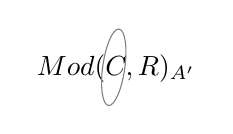
\begin{tikzpicture}[baseline=(m.base)]
\node (m) at (0,0) {$\operatorname{Mod}(\uuline{C},R)_{A'}$};
\handwritten{\draw[gray] (-.03,.02) ellipse [x radius=.14,y radius=.49,rotate=-8];}
\end{tikzpicture}}
(pour $A'$ \deleted{anneau} \deleted{affine d'un ouvert affine de $S=\operatorname{Spec}(A)$)}\inserted{une $A$-algèbre)} est équivalente à la catégorie fibrée des sections de $\uline{C}$ munis d'une opération de $R$\unsure{n|.} \unsure{En|Bn} particulier, sa restriction au \deleted{site} petit site zariskien affine de $S$ \deleted{\unsure{site|sitd}} s'identifie à
\figure{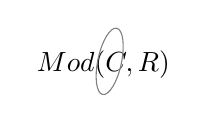
\begin{tikzpicture}[baseline=(m.base)]
\node (m) at (0,0) {$\operatorname{Mod}(\uline{C},R)$};
\handwritten{\draw[gray] (.08,.04) ellipse [x radius=.15,y radius=.43,rotate=-12];}
\end{tikzpicture}}
; c'est donc un champ si $\uline{C}$ en est un, donc $\operatorname{Mod}(R,\unsure{\mathbb{C}|\mathbb{A}})$ est localisable \inserted{sur $S$} si $C$ l'est.

NB\quad Si $R$ est commutatif, $\operatorname{Mod}(R,C)$ est même $R$-linéaire. Notre raisonnement \uline{ne prouve pas} que \deleted{$C$ est} $\operatorname{Mod}(R,C)$ est local\deleted{\unsure{r|i}}isable sur $R$ i.e. sur $\operatorname{Spec}(R)$ (ce qui est plus fort que de dire qu'elle est localisable sur $S=\operatorname{Spec}(A)$).

d)\quad \deleted{Deux objets \unsure{de} $\unsure{X,Y|X;Y}$ de $C$ \unsure{tels que} sont dits} Si $C$ est localisable sur $A$, alors pour $A'$ \deleted{ouvert} anneau affine d'un ouvert affine \inserted{$U$} de $S$, $C_{A'}$ est localisable sur $A'$, et le champ associé sur $U$ s'identifie à la restriction \unsure{du|de} champ $\uline{C}$ à $U$.

e)\quad Deux objets de $C$ sont dits apparentés (ou $A$-apparentés) s'ils sont localement isomorphes sur $A$. \unsure{C'est|D'est} évidemment une relation déquivalence, et la sous-catégorie pleine de $C$ formée des objets apparentés à un objet de $C$ est une catégorie \deleted{de} $A$-linéaire localisable sur $A$, et c'est une catégorie de Deuring,
% archive sheet number: 81

\scanpage{136}
\begin{flushright}1.4.68\end{flushright}
\margin{\handwritten{\unsure{4|V}}}

\uline{D I V E R S}

\uline{CANDIDATS}

.\quad TAFT

.\quad Scientifiques Russes

-\quad A la demande de M. MICHEL, revoir les dossiers de :

DASGUPTA

OKABAYASHI

ROCKMORE

SHIMA

SOMMER

YOKOO

\diagram{$\begin{array}{lll}
\text{-\quad Suggestion M. MICHEL\quad :} & ( & \text{polonais}\\
 & ) & \text{indiens}
\end{array}$}
% archive sheet number: 135

\scanpage{170}
\uline{Foncteurs \unsure{fibres|fibrés} motiviques, et gps fondamen\unsure{taux} motiviques.}

À examiner :

0)\quad VA
\figure{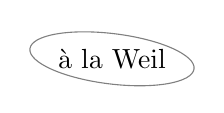
\begin{tikzpicture}[baseline=(w.base)]\node (w) at (0,0) {à la Weil};\draw[gray] (0,0) ellipse [x radius=1.05,y radius=.32,rotate=-7];\end{tikzpicture}}
\unsure{associées} aux motifs purs de poids impairs sur
\inserted{Conditions de Hodge-Riemann\ldots}

\margin{OK\quad *}
\figure{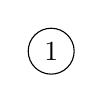
\begin{tikzpicture}\node[draw,circle,inner sep=3pt] {1};\end{tikzpicture}}
Extension du groupe \unsure{définie|définies|défini} par des \unsure{places arithmétiques|places antiques}

\uline{Groupe fondamental motivique.}

\figure{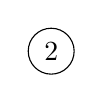
\begin{tikzpicture}\node[draw,circle,inner sep=3pt] {2};\end{tikzpicture}}
Relations avec le corps de classes

\margin{OK}
\figure{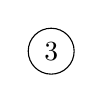
\begin{tikzpicture}\node[draw,circle,inner sep=3pt] {3};\end{tikzpicture}}
Cas du spectre d'un corps fini. Pb \unsure{motivique}

\unsure{parties|positives} à \unsure{val.} dans $\mathbb{R}$ ???

\margin{*}
4)\quad Rôle du groupe fondamental motivique pour la comparaison des réseaux canoniques
\diagram{$\left[\begin{array}{ll}
\text{des \unsure{Ch.|Coh.} de Hodge} & \left|\begin{array}{l}
\text{2 réseaux \unsure{transcendant|transcendants} \unsure{pr.|prov.} des places diff.}\\
\text{réseau transcendant et \unsure{réseau|réseaux} de Hodge}
\end{array}\right.\\[1em]
\text{des Coh. $l$-adique} & \left|\text{2 réseaux transcendants}\right.
\end{array}\right]$}

5)\quad Relations \inserted{de 4} avec \unsure{mes|les} \unsure{autres} \unsure{anciens|axiomes}

6)\quad Fonctions $L$: équation fonctionnelle

\margin{OK}
7)\quad Structures \unsure{pratiques|positives|p-adiques}\ldots

\deleted{\unsure{7}}8)\quad Topologie à mettre sur $\mathbb{Z}$ \texttt{-{}-{}-{}-}

9)\quad Hyp. de Riemann \unsure{??}

\margin{Positivité à la Hodge en se ramenant à des questions de \uline{diviseurs} par \unsure{éclatements}, ou variétés de drapeaux ??}
% archive sheet number: 169

\scanpage{171}
\mspage{20}
SYSTÈMES de RACINES\hfill Tribu n$^{\handwritten{o}}$ \handwritten{59}

de signe $+1$.

1) On pose $E=\unsure{I|\Gamma|\mathbb{P}|L|\Pi}\handwritten{/3}P$. C'est un $\uuline{F}_{\handwritten{3}}$-espace vectoriel de dimension 5. Montrer que le produit $(x,y)$ définit sur $E$ une forme bil. sym. non dégénérée. Montrer que deux éléments distincts de $R$ ont des images distinctes dans $E$.

2) On note $\operatorname{O}(E)$ le groupe orthogonal de $E$, muni de la forme bil. précédente. On a $\operatorname{O}(E)=\handwritten{\{\pm}1\handwritten{\}}\times\operatorname{SO}(E)$. La norme spinorielle définit un homomorphisme surjectif $\operatorname{SO}(E)\handwritten{\longrightarrow\{\pm}1\handwritten{\}}$ dont le noyau est noté $\operatorname{SO}^{\handwritten{+}}(E)$. Le groupe $\operatorname{SO}^{\handwritten{+}}(E)$ est simple, (d'ordre 25 920) ; le quotient $\operatorname{O}(E)/\operatorname{SO}^{\handwritten{+}}(E)$ est de type $(2,2)$. En déduire que $\operatorname{O}(E)$ contient un sous-groupe $\handwritten{\Omega}(E)$ d'indice 2 distinct de $\operatorname{SO}(E)$ et ne contenant pas $-1$ ; montrer que ce sous-groupe est unique.

3) Tout élément de $\operatorname{Aut}(R)$ définit par passage au quotient un élément de $\operatorname{O}(E)$. Montrer, (en comparant les ordres), que l'on obtient ainsi un isomorphisme de $\operatorname{Aut}(R)$ sur $\operatorname{O}(E)$ ; l'image de $W(R)$ par cet isomorphisme est $\handwritten{\Omega}(E)$, celle de $W^{\handwritten{+}}(R)$ est $\operatorname{SO}^{\handwritten{+}}(E)$.

(Ainsi, $W(R)$ est extension d'un groupe à deux éléments \unsure{oar|par} le groupe simple d'ordre 25 920).

F) Groupe de Weyl $W$ de $E_{\handwritten{7}}$.

Soient $Q$ le réseau radiciel, $P$ celui des poids. On a $2P\handwritten{\subset}Q$. Posons $E=Q\handwritten{/}2P$. La forme bilinéaire $(x\ y)$ définit, par passage au quotient, une forme bilinéaire sur le $F_{\handwritten{2}}$-espace vectoriel $E$, (noter que $(Q\mid 2P)\handwritten{\subset}2Z$). Montrer que cette forme est non dégénérée et alternée, (noter que $\dim(E)=\handwritten{6}$). En déduire un homomorphisme $W\handwritten{\longrightarrow}\operatorname{Sp}(E)=\operatorname{Sp}(3,F_{\handwritten{2}})$.

Montrer que la suite
\[
1\handwritten{\longrightarrow}(1,-1)\handwritten{\longrightarrow}W\handwritten{\longrightarrow}\operatorname{Sp}(3,F_{\handwritten{2}})\handwritten{\longrightarrow}1
\tag*{(s)}
\]
est exacte, (on peut utiliser le fait que $\operatorname{Sp}(3,F_{\handwritten{2}})$ est d'ordre $2^{\handwritten{9}}.3^{\handwritten{4}}.5.7$ ; cf. Alg. IX).

Montrer que le sous-groupe $W^{\handwritten{+}}$ formé des éléments de déterminant 1 de $W$ se projette isomorphiquement sur $\operatorname{Sp}(3,F_{\handwritten{2}})$, (noter que ce sous-groupe ne contient pas $-1$).

Donner une seconde démonstration de (s) en utilisant la structure de $W(E_{\handwritten{8}})$ et l'isomorphisme $\operatorname{Sp}(3,F_{\handwritten{2}})\handwritten{\longrightarrow}\uline{\operatorname{O}}(7,F_{\handwritten{2}})$.
% archive sheet number: 170

\scanpage{181}
% The printed list is upside down in the supplied scan; reading order follows the upright list.
\diagram{$\begin{array}{llllll}
\text{0170} & \text{TAULELLE} & \text{VERONIQUE} & \text{2740730007019} & \text{930728S} & \text{2A2} \\
\text{0171} & \text{TIGNY} & \text{SANDRINE} & \text{2710769383109} & \text{900477U} & \text{2A2} \\
\text{0172} & \text{TOURIERE} & \text{SOPHIE} & \text{2740434172243} & \text{942009J} & \text{2A2} \\
\text{0173} & \text{TRIAIRE} & \text{AGNES} & \text{2720934111012} & \text{910300B} & \text{2A2} \\
\text{0174} & \text{TRIAIRE} & \text{FRANCOISE} & \text{2720934111013} & \text{910299A} & \text{2A2} \\
\text{0175} & \text{TUFFERY} & \text{ISABELLE} & \text{2700534172087} & \text{931766V} & \text{2A2} \\
\text{0176} & \text{VALMALETTE} & \text{SOPHIE} & \text{2710778551110} & \text{941607X} & \text{2A2} \\
\text{0177} & \text{VEDEL} & \text{KARINE} & \text{2710643157065} & \text{911395S} & \text{2A2} \\
\text{0178} & \text{VERGER} & \text{ESTELLE} & \text{2730234172047} & \text{920133V} & \text{2A2} \\
\text{0179} & \text{VICART} & \text{DAVID} & \text{1720362119173} & \text{910910P} & \text{2A2} \\
\text{0180} & \text{VIDAL} & \text{CAROLE} & \text{2720434172236} & \text{910273X} & \text{2A2} \\
\text{0181} & \text{VILLAR} & \text{MAXIME} & \text{1700934032119} & \text{900007H} & \text{2A2} \\
\text{0182} & \text{WINTREBERT} & \text{CLAIRE} & \text{2730334172023} & \text{923054V} & \text{2A2} \\
\text{0183} & \text{WOUTERS} & \text{FREDERIQUE} & \text{2721059350782} & \text{920453T} & \text{2A2} \\
\end{array}$}

*****\quad FIN\quad LISTE\quad *****
% archive sheet number: 180

\scanpage{188}
\handwritten{\mspage{70}}
that there exists $n_{\handwritten{\unsure{o|0}}}(K)$ such that at $n\ \handwritten{\unsure{\mathrm{m}}}\ n_{\handwritten{o}}(K)$
\[
\handwritten{H^i(V,K[nE])=0\qquad i=1,2,\ldots}
\]

From the exact sequence
\[
\handwritten{H^i(V,O_V(-E_\varphi)[nE])\longrightarrow H^i(V,O_V[nE])\longrightarrow H^i(V,K[nE])}
\]
at $n\geq n_{\handwritten{o}}(K)$, $i=1,2,\ldots$ we obtain:
\[
\handwritten{\dim H^i(V,O_V[nE])\leq\dim H^i(V,O_V(-E_\varphi)[nE]).}
\]

Since
\[
\handwritten{O_V(-E_\varphi)\cong O_V[-E],}
\]
then
\[
\handwritten{O_V(-E_\varphi)[nE]\cong O_V[-E][nE]\cong O_V[(n-1)E].}
\]

Therefore, at $n\geq n_{\handwritten{o}}(K)$, $i=1,2,\ldots$
\[
\handwritten{\dim H^i(V,O_V[nE])\leq\dim H^i(V,O_V[[n-1]E]).}
\]

Evidently, there exists such $n'$ that, at $n\geq n'$
% archive sheet number: 187

